\documentclass[a4paper]{article}

%% Language and font encodings
\usepackage[english]{babel}
\usepackage[utf8x]{inputenc}
\usepackage[T1]{fontenc}

%% Sets page size and margins
\usepackage[a4paper,top=3cm,bottom=2cm,left=3cm,right=3cm,marginparwidth=1.75cm]{geometry}

%% Useful packages
\usepackage{amsmath}
\usepackage{amsfonts}
\usepackage{booktabs}

\usepackage{graphicx}
\usepackage{tikz}
\usetikzlibrary{arrows.meta}

\usepackage[colorinlistoftodos]{todonotes}
\usepackage[colorlinks=true, allcolors=blue]{hyperref}

\usepackage{color}
\usepackage{url}

%% display solutions or not
\newif\ifsol
\soltrue % comment out to hide solutions

\title{Section 8: HMMs}
\author{CS 182 - Artificial Intelligence}
\date{}

\begin{document}
\maketitle

\section*{Probability Review}

A {\bf{random variable}} $X$ is a variable which could take on various values with specified probabilities (its distribution). Two random variables $X$ and $Y$ are independent if $p(x, y) = p(x)p(y)$. Then, the probability of an event that depends on both $X$ and $Y$ (for example, the event that $X == 1$ and $Y == 2$) will be given by a value in the {\bf{joint probability distribution}} $p(x, y)$. \\

\noindent The {\bf{marginal probability distribution}} is the probability distribution of a subset of variables from a {\bf{joint probability distribution}}. For example, the marginal probability distribution $p(y)$ can be found by summing across all values of $x$ in $p(x, y)$:
\begin{align*}
p(x) = \sum_{y \in \mathcal{Y}} p(x, y) \\
p(x) = \int_{\mathcal{Y}} p(x,y) dy
\end{align*}

\noindent When we know that an event $B$ has happened, that could influence the probability of another event $A$. The new probability of $A$ given $B$ is the {\bf{conditional probability}} $P(A|B)$. If $B$ changes the distribution of a random variable $X$, we write the new random variable as $X|B$, and the new distribution $P(X|B)$ is the conditional distribution:
$$ P(A | B) = \frac{P(A \;\; \text{and} \;\; B)}{P(B)}$$

\noindent Note that this has some direct implications: for instance, if $A$ is the event $X == x$ and $B$ is the event $Y == y$, we have an expression relating distributions (sometimes called the {\bf{product rule}}):
$$ p(x | y) = \frac{p(x, y)}{p(y)}$$
which implies that
$$ p(x, y) = p(x | y) p(y) = p(y | x) p(x)$$

\noindent Finally, you may have heard of {\bf{Bayes' Theorem}} (also known as {\bf{Bayes' Rule}} or {\bf{Bayes' Law}}), a very prominent statement that relates conditional probabilities between events:
$$ p(x | y) = \frac{p(y | x) p(x)}{p(y)} $$ \\
In machine learning, we are often looking for parameters $\theta$ based on the distribution of data $y$. Then, we interpret $p(\theta)$ as the {\bf{prior}} (the distribution of $\theta$ without knowing about $y$), $p(y)$ as the {\bf{evidence}} (the overall probability of this data without considering our parameters), $p( y | \theta)$ as the {\bf{likelihood}} (how likely are we to collect this data given the parameters?) and $p( \theta | y)$ as the {\bf{posterior}} (the distribution of $\theta$ after knowing about $y$).
\begin{align*}
\underbrace{p(\theta | y)}_{\text{posterior}}
&= \frac{\overbrace{ p(y | \theta) }^{\text{likelihood}} 
	\overbrace{ p(\theta) }^{\text{prior}}}
{\underbrace{p(y)}_{\text{evidence}}}
\end{align*}

\section*{Markov Models}
\noindent A Markov model shows the probabilistic transitions of a \textbf{state} $X$. The system must obey the {\bf{Markov assumption}} that the conditional probability distribution of future states of the process (conditional on both past and present states) depends only upon the present state:
\[
P(X_T|X_1, \ldots, X_{T-1}) = P(X_T|X_{T-1}).
\]
And therefore all we need to fully define the model is:
\begin{itemize}
    \item An initial distribution $P(X_0)$
    \item Transition probabilities $P(X_{t}|X_{t-1})$
\end{itemize}
Furthermore, we can express the probability of a sequence of states as
\[
P(X_1, \ldots, X_T) = P(X_1) \prod_{t=2}^T P(X_t|X_{t-1})
\]
Note that as $t$ becomes large, the probabilities $P(X_t)$ will converge to a \textbf{stationary distribution} regardless of the initial distribution $P(X_1)$. We can think of this as uncertainty growing over time. \\ 

\noindent We can now think of a Markov model as a generalization of an MDP that is embedded in probability distributions over actions. The statement that $P(X_T|X_1, \ldots, X_{T-1}) = P(X_T|X_{T-1})$ is the same as saying that all transitions only depend on the current state over random actions $T(s, a, s')$. Again we have a starting state and potentially a terminal state, or absorbing state. We could also have a Markov Model give off rewards at states although general Markov Models do not need to have rewards.

\section*{Hidden Markov Models}

In Hidden Markov Models (HMMs), you can no longer directly observe the state itself. You can only observe (noisy) emissions $e$ from those states. Unlike in RL, where we were no longer able to know the transition probabilities, here we don't know the actual value of the state at each time. Thus, an HMM is defined by the following:
\begin{enumerate}
\item An initial distribution $P(X_1)$
\item Transition probabilities $P(X_{t}|X_{t-1})$
\item Emission probabilities $P(E_t|X_t)$
\end{enumerate}
We can use those to compute the joint distribution
\[
P(X_1, E_1, \ldots, X_T, E_T) = P(X_1) P(E_1|X_1) \prod_{t=2}^T P(X_{t}|X_{t-1}) P(E_t|X_t)
\]
Finally, we can define the \textbf{belief} at time $t$ as the probability of being in a specific state given all of the evidence seen so far:
\[
B_t(x) = P(X_t=x|e_{1:t}).
\]
We can therefore solve for our belief of the state throughout time (\textbf{filtering}) through the \textbf{forward algorithm} by updating for (1) the passage of time and (2) receiving/observing new evidence:
\begin{enumerate}
\item $P(x_t|e_{1:t-1}) = \sum_{x_{t-1}} P(x_{t-1}|e_{1:t-1}) \cdot P(x_t|x_{t-1})$
\item $P(x_t|e_{1:t}) \propto P(x_t|e_{1:t-1}) \codt P(e_t|x_t)$
\end{enumerate}
These equations can be derived by applying Bayes rule, the chain rule, and conditional independence to the definition of the belief at each time step under the HMM model. There is also a MDP equivalent for HMM which are called POMDPs and these are some of the hardest problems to solve in robotics due to the large state spaces and uncertainty. \textbf{Particle Filters} are designed to attempt to overcome this issue of needing to explicitly write out the belief distribution across all states by instead tracking a series of particles to compute a discrete, sample-based, approximation of the belief distribution. Particles are passed through a transition model for the elapse time step and then weighted based on the emissions seen in the observe step. Particles are then resampled according to this distribution to normalize before the process is repeated.

\clearpage
\section*{Practice Problems}

\begin{enumerate}
    \item Suppose you have a Markov Process defined by the following table:
        \begin{figure}[h]
            \centering
            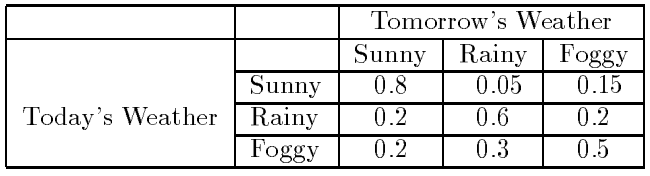
\includegraphics[width=.5\textwidth]{figs/sunny-foggy}
        \end{figure}
        
    \begin{enumerate}
        \item Transform the table into a finite state automaton representation.\\
        \ifsol
            \begin{figure}[h]
                \centering
                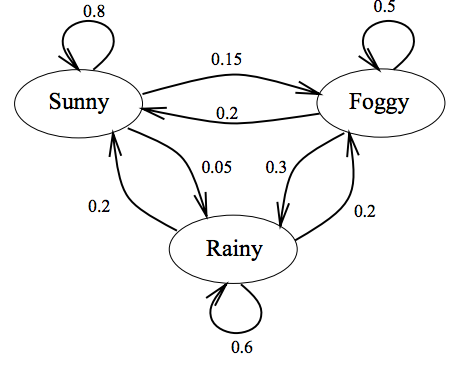
\includegraphics[width=.45\textwidth]{figs/1-sol}
            \end{figure}
        \else
            \bigskip \bigskip \bigskip \bigskip \bigskip \bigskip \bigskip \bigskip \bigskip \bigskip \bigskip \bigskip \bigskip \bigskip \bigskip
        \fi
        \item Given that today is \emph{sunny}, what is the probability that the next two days are first \emph{sunny} and then \emph{rainy}?
            \ifsol
                \textcolor{blue}{\begin{align*}
                P(X_2 = s, X_3 = r | X_1 = s) &= P(X_1=s) * P(X_2=s|X_1=s) * P(X_3=r|X_2=s) \\
                							  &= P(X_2=s|X_1=s) * P(X_3=r|X_2=s) \\
                                              &= 0.05 * 0.8 \\
                                              &= 0.04
                \end{align*}}
            \else
                \bigskip \bigskip \bigskip \bigskip \bigskip \bigskip \bigskip \bigskip \bigskip
            \fi
        \item Given that today is foggy, what is the probability that it rains in two days? \\
        \ifsol
            \textcolor{blue}{ 
            All three possibilities for $X_2$ can lead from $X_1=f$ to $X_3=r$. Therefore, we sum:
            \begin{align*}
            P(X_3=r|X_1=f) &=                     P(X_2=f | X_1=f) * P(X_3=r|X_2=f) +\\
                           &\mathrel{\phantom{=}} P(X_2=r | X_1=f) * P(X_3=r|X_2=r) +\\
                           &\mathrel{\phantom{=}} P(X_2=s | X_1=f) * P(X_3=r|X_2=s) \\
                           &= 0.3 * 0.5 + 0.6*0.3 + 0.05 * 0.2 \\
                           &= 0.34
            \end{align*}}
        \else
            \bigskip \bigskip \bigskip \bigskip \bigskip \bigskip \bigskip \bigskip \bigskip
        \fi
        
        \item Suppose today is foggy weather. What is the probability of all possible weather in two days? \\
        \ifsol
            \textcolor{blue}{\begin{table}[h]
            \centering
            \begin{tabular}{@{}lllll@{}}
            \toprule
              & $X_1$ & $X_2$ & $X_3$                           &  \\ \midrule
            s & 0.0   & 0.2   & 0.2*0.80+0.3*0.2+0.5*0.2 = 0.32  &  \\
            r & 0.0   & 0.3   & 0.2*0.05+0.3*0.6+0.5*0.3 = 0.34 &  \\
            f & 1.0   & 0.5   & 0.2*0.15+0.3*0.2+0.5*0.5 = 0.34 &  \\ \bottomrule
            \end{tabular}
            \end{table}}
        \else
            \bigskip \bigskip \bigskip \bigskip \bigskip \bigskip \bigskip \bigskip \bigskip
        \fi
    \end{enumerate}
    
    \clearpage
    \item Imagine you are a computer scientist and therefore do not leave your basement, ever. Now, the only evidence for the weather is whether the person who brings your daily meal carries an umbrella. You know the following emission probabilities $E$:\\
    \begin{figure}[h]
        \centering
        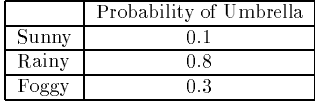
\includegraphics[width=.4\textwidth]{figs/umbrella}
    \end{figure}

    Yesterday, you were forced to go outside because of a fire drill -- the worst -- and saw that it was sunny. Today, your caregiver has an umbrella on them. What it is the probability that it is raining today? 
    
    \ifsol
        \textcolor{blue}{ We need to marginalize over all the probabilities of seeing an umbrella \begin{align*}
        \frac{p(X_2=r|X_1=s)p(E_2=u|X_2=r)}{p(E_2=u|X_1=s)} &= \frac{p(X_2=r|X_1=s)p(E_2=u|X_2=r)}{\sum_{i \in [s,r,f]} p(E_2=u|X_2=i) p(X_2=i|X_1=s)} \\
            &= \frac{0.05 * 0.8}{0.8*0.1 + 0.05*0.8 + 0.15*0.3} \\
            &\approx 0.2424
        \end{align*}}
    \else
        \bigskip \bigskip \bigskip \bigskip \bigskip \bigskip \bigskip \bigskip
    \fi
    
    \item Now consider the following conditional probabilities. 
        \begin{figure}[h]
        \centering
        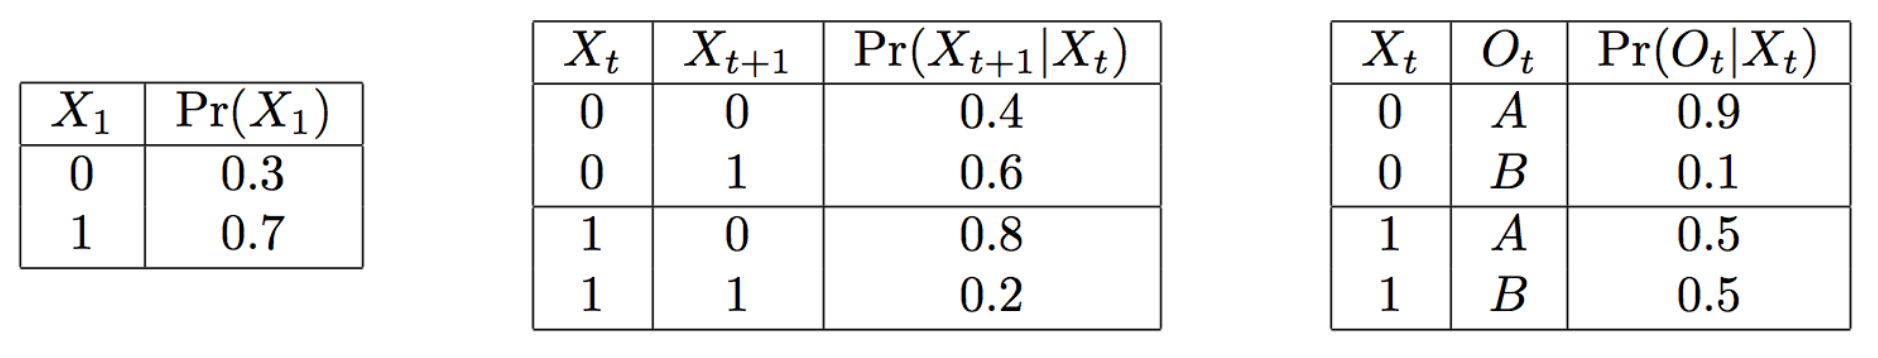
\includegraphics[width=0.8\textwidth]{figs/hmmtask2.png}
        \end{figure}
        
        \begin{enumerate}
            \item Draw the full HMM model for this set of probabilities:\\
            \ifsol
                \begin{center}
                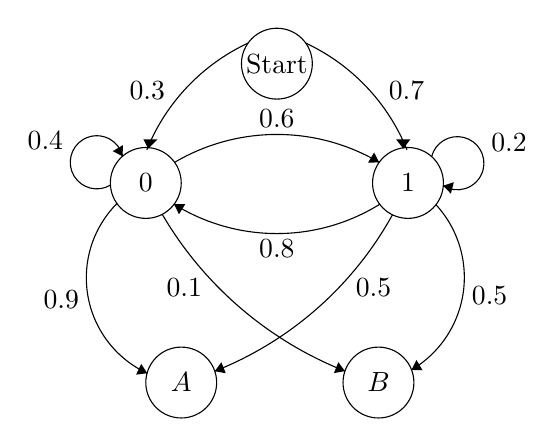
\begin{tikzpicture}[scale=0.15]
                \tikzstyle{every node}+=[inner sep=0pt]
                \draw [black] (37.7,-7) circle (3);
                \draw (37.7,-7) node {Start};
                \draw [black] (26.6,-17.1) circle (3);
                \draw (26.6,-17.1) node {$0$};
                \draw [black] (48.8,-17.1) circle (3);
                \draw (48.8,-17.1) node {$1$};
                \draw [black] (29.6,-34) circle (3);
                \draw (29.6,-34) node {$A$};
                \draw [black] (46.3,-34) circle (3);
                \draw (46.3,-34) node {$B$};
                \draw [black] (40.137,-5.257) arc (65:22:17);
                \fill [black] (47.8,-13.41) -- (48.4,-14.2) -- (49.0,-13.41);
                \draw (47.137,-9.257) node [right] {$0.7$};
                \draw [black] (35.263,-5.257) arc (-65:-22:-17);
                \fill [black] (26.4,-13.41) -- (26.8,-14.2) -- (27.6,-13.41);
                \draw (28.263,-9.257) node [left] {$0.3$};
                \draw [black] (29.037,-15.357) arc (120.52398:59.47602:17.056);
                \draw (37.7,-12.49) node [above] {$0.6$};
                \draw [black] (46.408,-18.904) arc (-58.17768:-121.82232:16.515);
                \fill [black] (28.99,-18.9) -- (29.41,-19.75) -- (29.94,-18.9);
                \draw (37.7,-21.89) node [below] {$0.8$};
                \draw [black] (50.797,-14.877) arc (165.80141:-122.19859:2.25);
                \fill [black] (46.36,-15.36) -- (45.93,-14.52) -- (45.42,-15.38);
                \draw (55.81,-13.71) node [right] {$0.2$};
                \fill [black] (51.78,-17.33) -- (52.43,-18.01) -- (52.68,-17.04);
                \draw [black] (23.617,-17.277) arc (301.12921:13.12921:2.25);
                \draw (19.64,-13.54) node [left] {$0.4$};
                \fill [black] (24.64,-14.84) -- (24.66,-13.9) -- (23.8,-14.41);
                \draw [black] (26.72,-33.212) arc (-114.93875:-224.92927:8.916);
                \fill [black] (26.72,-33.21) -- (26.21,-32.42) -- (25.78,-33.33);
                \draw (20.98,-26.94) node [left] {$0.9$};
                \draw [black] (51.159,-18.931) arc (42.7293:-59.55867:9.087);
                \fill [black] (49.09,-32.93) -- (50.03,-32.96) -- (49.52,-32.09);
                \draw (54.17,-26.61) node [right] {$0.5$};
                \draw [black] (43.463,-33.029) arc (-111.62882:-149.62165:31.312);
                \fill [black] (43.46,-33.03) -- (42.9,-32.27) -- (42.53,-33.2);
                \draw (29.86,-25.18) node [below] {$0.1$};
                \draw [black] (47.485,-19.795) arc (-28.90492:-68.38608:29.67);
                \fill [black] (32.44,-33.04) -- (33.37,-33.21) -- (33,-32.28);
                \draw (45.88,-25.18) node [below] {$0.5$};
                \end{tikzpicture}
                \end{center}
            \else
                \bigskip \bigskip \bigskip \bigskip \bigskip \bigskip \bigskip \bigskip \bigskip \bigskip \bigskip
            \fi
            \item Suppose that $O_1 = A$ and $O_2 = B$ is observed. Use the Forward algorithm to compute the probability distribution $p(X2| O1 = A, O2 = B) = B_2(X2)$.\\
            \ifsol
                \begin{tabular}{lll}
                \toprule
                $X_1$   & $Pr(X_1, O_1 = A)$ & Normalized \\ \midrule
                0       & 0.3 * 0.9 = 0.27 &  27/62 \\
                1       & 0.7 * 0.5 = 0.35 &  35/62 \\\bottomrule
                $X_2$   & $Pr(X_2, O_1 = A, O_2 = B)$ & Normalized \\ \midrule
                0       & 0.1 * [0.4 * 27/62 + 0.8 * 35/62] = 97/1550 &  97/387 $\approx$ 0.25 \\
                1       & 0.5 * [0.6 * 27/62 + 0.2 * 35/62] = 29/155 &  290/387 $\approx$ 0.75 \\ \bottomrule
                \end{tabular}
                % \begin{figure}[h]
                % \centering
                % 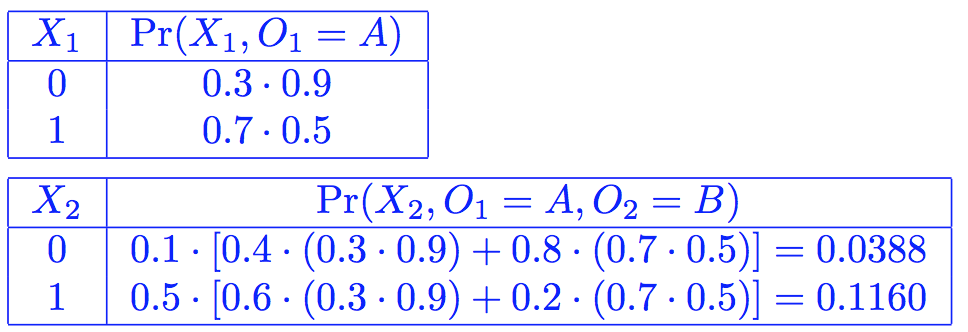
\includegraphics[width=0.5\textwidth]{figs/sol1}
                % \end{figure}
            \else
                \bigskip \bigskip \bigskip
            \fi
        \end{enumerate}
\end{enumerate}
\end{document}